\chapter{Random walk e algoritmo randomizzato per 2-SAT}

\section{La legge del disordine}

\scan{65}
Il riferimento è il libro divulgativo di George Gamow \emph{One, Two, Three\dots\ Infinity}
(1947), e in particolare il capitolo dedicato alla \emph{legge del disordine} (\emph{The Law
of Disorder}): anche da un comportamento completamente disordinato si riesce a estrarre una
legge quantitativa precisa.

L'esempio classico è il \emph{drunkard's walk}: un ubriaco $u$ parte da un lampione al centro
di una piazza e cammina senza meta, cambiando direzione a ogni passo in modo del tutto
casuale. È il prototipo di \textbf{random walk}; qui lo consideriamo in due dimensioni, su una
griglia.

\begin{figure}[H]
  \centering
  % ubriaco-griglia -- pag. 65
% Il "drunkard's walk" di Gamow: il piano xy visto in prospettiva (parallelogramma),
% i due lati obliqui fanno da assi cartesiani; al centro l'ubriaco u accanto al
% lampione da cui parte, e attorno il cammino irregolare (ellisse + curva tratteggiata).
% Il callout in alto a destra nomina la cosa: random walk, 2D su una griglia.
\begin{tikzpicture}[
    >=Latex,
    scale=0.95,
    font=\footnotesize,
    piano/.style={draw=black,line width=0.9pt},
    filo/.style={draw=black!75,line width=0.6pt},
    tratto/.style={draw=black!60,line width=0.7pt}]

  % ---- il piano (la piazza) in prospettiva ---------------------------------
  \coordinate (A) at (0.00,0.00);   % basso a sinistra
  \coordinate (B) at (4.00,0.00);   % basso a destra
  \coordinate (C) at (5.90,2.30);   % alto a destra
  \coordinate (D) at (1.90,2.30);   % alto a sinistra

  \draw[piano] (A) -- (B);
  \draw[piano] (D) -- (C);
  % lato AD prolungato oltre D: e' l'asse y
  \draw[piano,->] (A) -- (2.22,2.69);
  % lato BC con la punta di freccia a un terzo dell'altezza: e' l'asse x
  \draw[piano,postaction={decorate,decoration={markings,
        mark=at position 0.38 with {\arrow{Latex}}}}] (B) -- (C);

  \node[anchor=south east] at (2.16,2.66) {$y$};
  \node[anchor=north]      at (4.08,-0.10) {$x$};

  % ---- l'ubriaco ------------------------------------------------------------
  \draw[filo] (2.35,1.52) circle (0.13);            % testa
  \draw[filo] (2.35,1.39) -- (2.35,0.82);           % busto
  \draw[filo] (2.08,0.92) -- (2.35,1.25) -- (2.62,0.92);  % braccia
  \draw[filo] (2.35,0.82) -- (2.14,0.42);           % gambe
  \draw[filo] (2.35,0.82) -- (2.56,0.42);
  \node[anchor=east] at (2.00,1.20) {$u$};

  % ---- il lampione ----------------------------------------------------------
  \draw[filo,line width=1.0pt] (3.10,0.55) -- (3.10,1.76);
  \draw[filo] (3.10,2.32) -- (3.27,2.02) -- (3.10,1.72) -- (2.93,2.02) -- cycle;

  % ---- il cammino: prima l'orbita "regolare"... -----------------------------
  \draw[tratto,rotate around={10:(2.75,0.62)}] (2.75,0.62) ellipse (1.10 and 0.42);

  % ---- ...poi il vagabondaggio disordinato attorno ad essa -------------------
  \draw[tratto,densely dashed] plot[smooth cycle,tension=0.85] coordinates {
      (4.20,0.92) (3.96,1.32) (3.40,1.58) (2.70,1.66) (2.00,1.50) (1.38,1.18)
      (1.15,0.78) (1.35,0.42) (1.90,0.20) (2.60,0.14) (3.32,0.24) (3.96,0.50) };

  % ---- la domanda ------------------------------------------------------------
  \draw[filo,->] (2.45,0.02) to[out=-90,in=170] (3.52,-0.82);
  \node[anchor=west] at (3.60,-0.84) {\emph{arriver\`a a casa?}};

  % ---- il callout -------------------------------------------------------------
  \draw[filo] plot[smooth cycle,tension=0.85] coordinates {
      (8.45,3.32) (8.25,3.74) (7.58,3.94) (6.85,3.92) (6.15,3.70) (5.88,3.32)
      (6.18,2.94) (6.90,2.80) (7.72,2.82) (8.30,3.02) };
  \node at (7.15,3.36) {\textsf{random walk}};
  \draw[filo,->] (6.22,2.92) to[out=235,in=65] (5.96,2.40);
  \node[anchor=west] at (6.20,2.10) {($2$D su una griglia)};

\end{tikzpicture}

  \caption{Random walk in $2$D su una griglia: l'ubriaco $u$ parte dal lampione e vaga sul
  piano $xy$ seguendo un cammino del tutto irregolare. Arriverà a casa?}
\end{figure}

\begin{domanda}
L'ubriaco $u$ si allontanerà \emph{arbitrariamente} dal lampione?
\end{domanda}

La risposta è \textbf{sì}, e il conto che segue dice anche \emph{quanto}: dopo $N$ passi la
distanza dal lampione è dell'ordine di $\sqrt{N}$.

\begin{figure}[H]
  \centering
  % passo-griglia-2d -- pag. 65
% Un passo del random walk sulla griglia 2D: dal punto corrente si parte in una
% delle quattro direzioni cardinali, ciascuna con la stessa probabilita' p (=1/4).
% Le frecce non toccano il punto centrale, come nel manoscritto.
\begin{tikzpicture}[
    >=Latex,
    font=\footnotesize,
    passo/.style={line width=0.7pt,->}]

  % --- posizione corrente ---
  \fill (0,0) circle (1.5pt);

  % --- le quattro direzioni ---
  \draw[passo] (0, 0.20) -- (0, 1.00);
  \draw[passo] (0,-0.20) -- (0,-1.00);
  \draw[passo] ( 0.20,0) -- ( 1.00,0);
  \draw[passo] (-0.20,0) -- (-1.00,0);

  % --- probabilita', tutte uguali ---
  \node[anchor=west]  at ( 0.10, 1.00) {$p$};
  \node[anchor=north] at ( 1.00,-0.08) {$p$};
  \node[anchor=north] at (-1.00,-0.08) {$p$};
  \node[anchor=east]  at (-0.10,-1.00) {$p$};

\end{tikzpicture}

  \caption{Un passo del random walk sulla griglia bidimensionale: dal punto corrente ci si
  sposta in una delle quattro direzioni, ciascuna con la stessa probabilità $p$ (dunque
  $p = 1/4$).}
\end{figure}

Siano $x_i$ e $y_i$ le proiezioni sui due assi dell'$i$-esimo tratto, con segno positivo o
negativo a seconda del verso in cui l'ubriaco si muove lungo quell'asse. Se $R$ è la distanza
dal lampione dopo $N$ passi, per il teorema di Pitagora
\[
  R^{2} \;=\; (x_1 + x_2 + \dots + x_N)^{2} \;+\; (y_1 + y_2 + \dots + y_N)^{2}.
\]

Sviluppiamo il primo quadrato:
\begin{align*}
  (x_1 + x_2 + \dots + x_N)^{2}
    &\;=\; (x_1 + x_2 + \dots + x_N)\,(x_1 + x_2 + \dots + x_N)\\[2pt]
    &\;=\; x_1^{2} + x_2^{2} + x_3^{2} + \dots + x_N^{2}\\[4pt]
    &\qquad\;+\; 2\underbrace{\bigl(x_1x_2 + \dots + x_1x_N + x_2x_3 + \dots + x_{N-1}x_N\bigr)}_{\text{prodotti misti}} .
\end{align*}

\begin{osservazione}
Per ogni termine misto $x_i x_j$, al crescere di $N$ troverò lo stesso termine con segno
opposto con probabilità che tende a $1$: i passi sono indipendenti ed è ugualmente probabile
che la proiezione di un tratto sia positiva o negativa, quindi i prodotti misti si compensano
a due a due. Restano solo i quadrati, che sono tutti positivi.
\end{osservazione}

Dunque
\begin{align*}
  (x_1 + x_2 + \dots + x_N)^{2} &\;\longrightarrow\; x_1^{2} + x_2^{2} + \dots + x_N^{2} \;\approx\; N X^{2},\\
  (y_1 + y_2 + \dots + y_N)^{2} &\;\longrightarrow\; y_1^{2} + y_2^{2} + \dots + y_N^{2} \;\approx\; N Y^{2},
\end{align*}
dove $X^{2}$ e $Y^{2}$ denotano i valori medi di $x_i^{2}$ e di $y_i^{2}$, cioè le lunghezze
\emph{quadratiche} medie delle proiezioni di un passo, rispettivamente sull'asse $x$ e
sull'asse $y$. Sostituendo,
\[
  R \;=\; \sqrt{N\,(X^{2} + Y^{2})}
    \;=\; \sqrt{N}\cdot\underbrace{\sqrt{X^{2} + Y^{2}}}_{=\,1}
    \;=\; \sqrt{N},
\]
perché sulla griglia ogni passo ha lunghezza unitaria, cioè $x_i^{2}+y_i^{2}=1$ a ogni passo,
e dunque $X^{2}+Y^{2}=1$.

\begin{osservazione}
L'argomento della cancellazione è euristico: i prodotti misti non si annullano
algebricamente, quello che si annulla è il loro \emph{valore atteso}. Essendo i passi
indipendenti e a media nulla, $\E[x_i x_j] = \E[x_i]\,\E[x_j] = 0$ per $i \neq j$, e quindi
$\E[R^{2}] = N\bigl(\E[x^{2}] + \E[y^{2}]\bigr)$. Il $\sqrt{N}$ che si ottiene è perciò la
distanza \emph{quadratica media} $\sqrt{\E[R^{2}]}$, non la distanza «più probabile». Il
fatto qualitativo, che è quello che ci servirà, resta: la distanza cresce come $\sqrt{N}$ e
non come $N$.
\end{osservazione}

Il random walk, però, non ci interessa solo come curiosità fisica. Dal punto di vista
algoritmico la proprietà cruciale è un'altra: una passeggiata aleatoria è una \emph{visita} di
un grafo che non richiede di ricordare quali nodi siano già stati visitati, perché bastano la
posizione corrente e una sorgente di bit casuali. Nel resto del capitolo sfrutteremo
esattamente questo per ottenere un algoritmo per 2-SAT che lavora in spazio lineare nel numero
di variabili, laddove l'algoritmo deterministico costruisce e visita esplicitamente un grafo.

\section{SAT, 3-SAT, 2-SAT}

\scan{66}
Richiamiamo gli ingredienti del \emph{calcolo proposizionale}:
\[
\text{calcolo proposizionale}\quad
\begin{cases}
P,\; Q,\; R,\; X,\;\dots & \text{simboli proposizionali, con valori } 0/1,\\[6pt]
\wedge \qquad \vee \qquad \neg & \text{connettivi.}
\end{cases}
\]
Combinando simboli proposizionali e connettivi si ottengono le \emph{formule}, che possono
contenere variabili \emph{libere}; ammettendo anche i quantificatori $\forall$ ed $\exists$
sulle variabili proposizionali, una formula in cui nessuna variabile resta libera si dice
\emph{enunciato}.

\begin{esempio*}
\[
\forall Q\;\forall R\;\exists P\;\bigl[(P\wedge Q)\vee(\neg R\vee Q\vee\neg P)\bigr]
\]
è un enunciato: nessuna variabile resta libera. Formule di questa forma si chiamano
\emph{Quantified Boolean Formulae}; il problema di deciderne la verità si indica con QBF ed è
$\PSPACE$-completo.
\end{esempio*}

\begin{osservazione}
Passare da SAT (che è $\NP$-completo) alla sua versione \emph{quantificata} fa salire la
complessità da $\NP$ a $\PSPACE$: QBF è completo per $\PSPACE$, e sarebbe $\NP$-completo solo
se fosse $\NP = \PSPACE$.
\end{osservazione}

I tre problemi che ci interessano si scrivono allora nella forma seguente, in cui tutte le
variabili sono quantificate \emph{esistenzialmente}:
\[
\left\{
\begin{array}{l@{\qquad}l@{\quad}l}
\text{SAT}   & \exists x_1,\dots,x_n & \varphi\\[10pt]
\text{3-SAT} & \exists x_1,\dots,x_n &
   \displaystyle\bigwedge_{j=1}^{K}\bigl(\ell^{j}_{1}\vee \ell^{j}_{2}\vee \ell^{j}_{3}\bigr)\\[16pt]
\text{2-SAT} & \exists x_1,\dots,x_n &
   \displaystyle\bigwedge_{j=1}^{K}\bigl(\ell^{j}_{1}\vee \ell^{j}_{2}\bigr)
\end{array}
\right.
\]
dove ogni $\ell^{j}_{i}$ è un \emph{letterale}, cioè una variabile proposizionale oppure la
sua negazione, e $K$ è il numero di clausole dell'istanza; come d'uso, in $k$-SAT si richiede
che ogni clausola abbia \emph{al più} $k$ letterali, e i display qui sopra ne mostrano il caso
pieno. Le tre famiglie di istanze sono incluse l'una nell'altra,
\[
\text{2-SAT}\ \subseteq\ \text{3-SAT}\ \subseteq\ \text{SAT},
\]
perché una clausola di due letterali è in particolare una clausola di al più tre letterali, e
una congiunzione di clausole è in particolare una formula. In tutti e tre i casi si tratta del
\textbf{problema della soddisfacibilità} (per formule oppure per enunciati) di un dato tipo.

\paragraph{Versioni quantificate.}
Rimuovendo il vincolo che il prefisso sia puramente esistenziale, e ammettendo un'alternanza
arbitraria di $\forall$ ed $\exists$, si ottengono le corrispondenti versioni quantificate
\[
\text{QBF}\qquad \text{3-QBF}\qquad \text{2-QBF}.
\]

\begin{definizione}[Soddisfacibilità]
Risolvere un problema di soddisfacibilità significa cercare un \emph{assegnamento} di valori
di verità (cioè di valori $0/1$) alle variabili proposizionali che compaiono nella formula, in
modo da renderla vera.
\end{definizione}

\subsection{Forme normali}

Due forme normali ricorrenti per le formule proposizionali:
\begin{itemize}
  \item \textbf{CNF} (\emph{conjunctive normal form}): congiunzione di disgiunzioni di
        letterali;
  \item \textbf{DNF} (\emph{disjunctive normal form}): disgiunzione di congiunzioni di
        letterali.
\end{itemize}

\scan{67}
Il problema SAT si affronta dunque portando la formula in una delle due forme normali:
\[
  \text{SAT}\;
  \begin{cases}
    \;\longrightarrow\;\text{CNF}\\[4pt]
    \;\longrightarrow\;\text{DNF}
  \end{cases}
\]

\begin{osservazione}
Leggendo $\vee$ come somma e $\wedge$ come prodotto, una CNF è un \emph{prodotto di somme}
mentre una DNF è una \emph{somma di prodotti}:
\[
  \underbrace{(a+b)\cdot(c+d)\cdots}_{\text{CNF}}
  \qquad\qquad
  \underbrace{(a\cdot b)+(c\cdot d)+\cdots}_{\text{DNF}}
\]
\end{osservazione}

Una CNF ha la forma
\[
  (\ell_1\vee\ell_2)\wedge(\ell_3\vee\ell_4\vee\ell_5)\wedge\cdots
  \qquad\text{ossia}\qquad
  \bigwedge_{j=1}^{K}\Bigl(\bigvee_{i=1}^{k_j}\ell^{j}_{i}\Bigr),
\]
dove gli $\ell^{j}_{i}$ sono letterali e clausole diverse possono avere lunghezze diverse
($k_1$, $k_2$, \dots).

Per portare una formula in CNF si potrebbe procedere per pura distributività --- la
«moltiplicazione» dell'analogia aritmetica --- ma questa strada va scartata, perché fa
esplodere esponenzialmente il numero di clausole. Poiché però interessa soltanto
l'\emph{equisoddisfacibilità}, e non l'equivalenza logica, conviene invece
\textbf{introdurre nuove variabili}.

\begin{esempio}[da DNF a CNF introducendo una variabile]
Si parta dalla DNF
\[
  (\varphi_1\wedge\varphi_2)\vee(\varphi_3\wedge\varphi_4),
\]
in cui $\varphi_1,\dots,\varphi_4$ sono letterali. Introdotta una variabile fresca $u$ si
scrive
\[
  \bigl((\varphi_1\wedge\varphi_2)\vee u\bigr)\wedge\bigl((\varphi_3\wedge\varphi_4)\vee\neg u\bigr)
\]
e, distribuendo il $\vee$ dentro ciascuna congiunzione,
\[
  \bigl((\varphi_1\vee u)\wedge(\varphi_2\vee u)\bigr)\wedge\bigl((\varphi_3\vee\neg u)\wedge(\varphi_4\vee\neg u)\bigr)
\]
cioè la CNF
\[
  (\varphi_1\vee u)\wedge(\varphi_2\vee u)\wedge(\varphi_3\vee\neg u)\wedge(\varphi_4\vee\neg u).
\]
In notazione aritmetica lo stesso passaggio si legge
\[
  (a\cdot b)+(c\cdot d)\;\rightsquigarrow\;(a+u)\cdot(b+u)\cdot(c+\bar u)\cdot(d+\bar u).
\]
Con più di due termini si ripete il trucco introducendo altrettante variabili fresche.
\end{esempio}

\begin{osservazione}
Le due formule non sono logicamente equivalenti (la seconda parla anche di $u$), ma sono
equisoddisfacibili: se è vera $\varphi_1\wedge\varphi_2$ basta porre $u=0$, se è vera
$\varphi_3\wedge\varphi_4$ basta porre $u=1$; viceversa, in ogni assegnamento che soddisfa la
CNF il valore di $u$ seleziona quale dei due termini deve risultare vero.
\end{osservazione}

\subsection{Da CNF a 3-CNF}

Lo stesso trucco permette di accorciare le clausole:
\[
  \text{CNF}\;\longrightarrow\;\text{3-CNF}.
\]
Una clausola con $k>3$ letterali
\[
  \cdots\wedge(\ell_1\vee\ell_2\vee\cdots\vee\ell_k)\wedge\cdots
\]
\[\Downarrow\]
si sostituisce con la catena
\[
  \cdots\wedge(\ell_1\vee\ell_2\vee u_1)\wedge(\neg u_1\vee\ell_3\vee u_2)\wedge(\neg u_2\vee\ell_4\vee u_3)
  \wedge\cdots\wedge(\neg u_{k-3}\vee\ell_{k-1}\vee\ell_k)\wedge\cdots
\]
in cui $u_1,\dots,u_{k-3}$ sono variabili fresche. Ogni clausola prodotta ha esattamente $3$
letterali, e da una clausola di lunghezza $k$ se ne ottengono $k-2$: la trasformazione è
lineare nella dimensione della formula e preserva la soddisfacibilità.

\subsection{Aspvall--Plass--Tarjan: il grafo delle implicazioni}

Per il caso binario esiste un algoritmo deterministico lineare:
\[
  \Oh(n)\qquad\text{per 2-QBF.}
\]
Il risultato di Aspvall--Plass--Tarjan riguarda le formule booleane quantificate la cui
matrice è in 2-CNF (2-QBF); il caso puramente esistenziale è 2-SAT. L'idea è leggere ogni
clausola binaria come una coppia di implicazioni:
\[
  (\ell_1\vee\ell_2)
  \qquad\text{si legge}\qquad
  \overline{\ell_1}\to\ell_2,\qquad \overline{\ell_2}\to\ell_1 .
\]
Raccogliendo gli archi generati da tutte le clausole si ottiene il \emph{grafo delle
implicazioni} $G$, sul quale si calcolano le componenti fortemente connesse (CFC).

\begin{figure}[H]
\centering
% grafo-implicazioni-2sat -- pag. 67
% Il grafo delle implicazioni G di Aspvall--Plass--Tarjan.  I nodi sono letterali
% (senza cerchio, come nel manoscritto); la clausola (l_1 v l_2) genera i due archi
%       not l_1 --> l_2      e      not l_2 --> l_1 .
% La macchia irregolare rappresenta l'intero grafo G; fuori, a destra, la sigla CFC
% (componenti fortemente connesse), che e' cio' che su G si va a calcolare.
\begin{tikzpicture}[
    >=Latex,
    font=\small,
    bordo/.style={draw=black!70,line width=0.8pt},
    arco/.style={->,line width=0.7pt}]

  % ---- contorno del grafo (curva chiusa irregolare) ------------------------
  \draw[bordo] plot[smooth cycle,tension=0.85] coordinates {
      (-2.80, 0.10) (-2.40, 0.90) (-1.55, 1.30) (-0.40, 1.42)
      ( 0.80, 1.35) ( 1.85, 1.18) ( 2.58, 0.70) ( 2.80, 0.12)
      ( 2.58,-0.45) ( 1.75,-1.00) ( 0.60,-1.30) (-0.10,-1.45)
      (-1.10,-1.25) (-2.05,-0.95) (-2.65,-0.45) };

  % ---- nome del grafo, appoggiato al bordo in alto a destra ----------------
  \node[anchor=south west] at (1.72,0.98) {$G$};

  % ---- clausola (l_1 v l_2): primo arco,  not l_1 --> l_2 ------------------
  \node (nl1) at (-0.60, 0.62) {$\overline{\ell_1}$};
  \node (l2)  at (-1.85, 0.50) {$\ell_2$};
  \draw[arco] (nl1) to[bend left=15] (l2);

  % ---- clausola (l_1 v l_2): secondo arco,  not l_2 --> l_1 ----------------
  \node (nl2) at (0.15,-0.78) {$\overline{\ell_2}$};
  \node (l1)  at (1.45,-0.36) {$\ell_1$};
  \draw[arco] (nl2) to[bend right=15] (l1);

  % ---- cio' che si calcola su G -------------------------------------------
  \node[anchor=west] at (3.05,0.05) {CFC};

\end{tikzpicture}

\caption{Il grafo delle implicazioni $G$: la clausola $(\ell_1\vee\ell_2)$ produce i due archi
$\overline{\ell_1}\to\ell_2$ e $\overline{\ell_2}\to\ell_1$. Su $G$ si calcolano le componenti
fortemente connesse (CFC).}
\end{figure}

\begin{osservazione}
Nel caso puramente esistenziale il criterio è il seguente: la 2-CNF è insoddisfacibile se e
solo se esiste una variabile $x$ tale che $x$ e $\neg x$ cadono nella stessa componente
fortemente connessa di $G$. Poiché le CFC si calcolano con una visita in tempo lineare, si
ottiene l'algoritmo $\Oh(n)$ annunciato; per il caso quantificato (2-QBF) al criterio va
aggiunta una condizione sull'ordine dei quantificatori.
\end{osservazione}

\section{Un algoritmo randomizzato per 2-SAT}

\scan{69}
Riepilogando, per il caso binario abbiamo due algoritmi deterministici:
\[
  \text{CNF}\qquad \text{3-CNF}\qquad \text{2-CNF}
  \;\begin{cases}
    \;\longrightarrow\ \text{Aspvall--Plass--Tarjan (2-QBF)} & \Oh(n)\\[4pt]
    \;\longrightarrow\ \text{risoluzione} & \Oh(n^{2})
  \end{cases}
\]
dove la seconda riga è la chiusura per risoluzione dell'insieme delle clausole binarie. Il
punto debole di entrambi è lo stesso: costruiscono in modo esplicito una struttura di
dimensione almeno lineare nel numero dei letterali --- il grafo delle implicazioni ha un nodo
per letterale, mentre l'insieme dei risolventi può arrivare a $\Th(n^{2})$ clausole.
Possiamo semplificare ulteriormente, e usare la \emph{randomness}.

\scan{68}
Sia data una formula in 2-CNF e se ne consideri una clausola:
\[
  \cdots\;\wedge\;(\ell_1\vee\ell_2)\;\wedge\;\cdots
\]
Si parte da un \emph{assegnamento $f$ di valori di verità} e si itera il passo seguente: se
$(\ell_1\vee\ell_2)$ \emph{non} è soddisfatta da $f$, si fa il \textsc{flip} di \emph{uno dei
due valori di verità}, scelto \emph{a caso} fra i due.

\begin{osservazione}
Supponiamo che la formula di partenza sia soddisfacibile e fissiamo un assegnamento $f^{*}$
che la soddisfa. Se sotto $f$ i due letterali $\ell_1$ ed $\ell_2$ valgono entrambi $\bot$
--- cioè se la clausola $(\ell_1\vee\ell_2)$ non è soddisfatta --- allora $f^{*}$ ne rende
vero almeno uno, e quindi $f$ ed $f^{*}$ differiscono su almeno una delle due variabili
coinvolte. Invertendone una scelta a caso, con probabilità almeno $\tfrac12$ ci si
«avvicina» ad $f^{*}$: precisamente, il numero
\[
  k \;=\; \#\set{i \;:\; f(x_i)=f^{*}(x_i)}
\]
di variabili su cui $f$ coincide con $f^{*}$ aumenta di $1$ con probabilità almeno
$\tfrac12$; altrimenti diminuisce di $1$.
\end{osservazione}

Misurando così la distanza dall'obiettivo, ogni passo dell'algoritmo diventa uno spostamento
di una posizione lungo la linea degli stati $0,1,\dots,n$, dove $n$ è il numero delle
variabili proposizionali: da $k$ si passa a $k-1$ oppure a $k+1$, e a $k+1$ con probabilità
almeno $\tfrac12$.

\begin{figure}[H]
\centering
% random-walk-linea-2sat -- pagg. 68 e 69 (i due schizzi rappresentano la stessa cosa
% e qui sono fusi in un'unica figura).
% La linea degli stati 0,1,...,n: lo stato k conta le variabili su cui l'assegnamento
% corrente f coincide con l'assegnamento soddisfacente fissato f*.  Ogni FLIP sposta
% di +-1, e a k+1 si va con probabilita' almeno 1/2; n e' lo stato di arresto.
\begin{tikzpicture}[
    >=Latex,
    font=\footnotesize,
    asse/.style={line width=0.7pt},
    tacca/.style={line width=0.7pt},
    stato/.style={circle,fill,inner sep=0pt,minimum size=3.2pt},
    salto/.style={->,line width=0.6pt}]

  % ---- asse degli stati ----------------------------------------------------
  \draw[asse,->] (-0.55,0) -- (7.40,0);

  % ---- gli stati -----------------------------------------------------------
  \node[stato] at (0.00,0) {};
  \node[stato] at (0.75,0) {};
  \node[stato] at (1.45,0) {};
  \node[stato] at (2.95,0) {};
  \node[stato] at (3.95,0) {};
  \node[stato] at (4.95,0) {};
  \node[stato] at (6.55,0) {};

  % ---- tacche che attraversano l'asse: origine, stato corrente, arresto ----
  \draw[tacca] (0.00,-0.30) -- (0.00,0.30);
  \draw[tacca] (3.95,-0.26) -- (3.95,0.26);
  \draw[tacca] (6.55,-0.22) -- (6.55,0.22);

  % ---- etichette, tutte sulla stessa linea di base --------------------------
  \node[anchor=north] at (0.00,-0.34) {$0$};
  \node[anchor=north] at (0.75,-0.34) {$1$};
  \node[anchor=north] at (1.45,-0.34) {$2$};
  \node[anchor=north] at (2.15,-0.34) {$\cdots$};
  \node[anchor=north] at (2.95,-0.34) {$k-1$};
  \node[anchor=north] at (3.95,-0.34) {$k$};
  \node[anchor=north] at (4.95,-0.34) {$k+1$};
  \node[anchor=north] at (5.85,-0.34) {$\cdots$};
  \node[anchor=north] at (6.55,-0.34) {$n$};

  % ---- il passo: da k si va a k-1 oppure a k+1 ------------------------------
  \draw[salto] (3.88,0.32) to[out=145,in=55] (3.00,0.18);
  \draw[salto] (4.02,0.32) to[out=35,in=125] (4.90,0.18);
  \node[anchor=west,font=\scriptsize] at (5.05,0.46) {$\ge \tfrac12$};

  % ---- che cosa conta n -----------------------------------------------------
  \node[anchor=north west,align=left,font=\scriptsize,text=black!70]
    at (6.90,-0.26) {$n$ variabili\\proposizionali};

\end{tikzpicture}

\caption{Il passo dell'algoritmo visto come passeggiata aleatoria sulla linea degli stati
$0,1,\dots,n$: dallo stato $k$ si passa a $k-1$ oppure a $k+1$, e a $k+1$ con probabilità
almeno $\tfrac12$. Qui $n$ è il numero delle variabili proposizionali e lo stato $k$ conta le
variabili su cui l'assegnamento corrente $f$ coincide con l'assegnamento soddisfacente
fissato $f^{*}$.}
\end{figure}

Posso quindi vedere la mia ricerca come una \emph{visita randomizzata} di un \emph{grafo
lineare} (cammino): scriviamo $L_m$ per il cammino con $m$ nodi, cosicché la linea degli stati
$0,1,\dots,n$ è $L_{n+1}$.

\begin{figure}[H]
\centering
% grafo-lineare-L4 -- il grafo lineare (cammino) L_4 (quaderno, pag. 69).
% Cammino orizzontale con 4 nodi e 3 archi di lunghezza uguale, senza etichette
% sui nodi; a destra, staccata e leggermente piu' in basso, l'etichetta $L_4$.
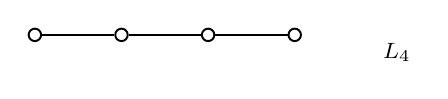
\begin{tikzpicture}[
    font=\footnotesize,
    nodo/.style={circle,draw,line width=0.7pt,fill=white,
                 inner sep=0pt,minimum size=4.5pt},
    arco/.style={line width=0.7pt}]

  % --- i quattro nodi del cammino, equispaziati ---
  \foreach \i in {0,1,2,3}{
    \node[nodo] (v\i) at (\i*1.1,0) {};
  }

  % --- i tre archi ---
  \draw[arco] (v0) -- (v1);
  \draw[arco] (v1) -- (v2);
  \draw[arco] (v2) -- (v3);

  % --- etichetta del grafo ---
  \node[anchor=west] at (4.3,-0.22) {$L_4$};

\end{tikzpicture}

\caption{Il grafo lineare $L_4$: il cammino con $4$ nodi e $3$ archi.}
\end{figure}

Il guadagno rispetto agli algoritmi deterministici è tutto nello spazio: basta infatti tenere
in memoria l'assegnamento corrente, un bit per variabile, e non serve alcuna traccia dei nodi
già visitati.
\begin{center}
\fbox{\textsc{spazio}\quad $\Oh(n)$ bit}
\end{center}

Per il tempo, vedremo che il numero atteso di passi necessari a percorrere tutta la linea è
\[
  \Oh(n^{2}),
\]
e che il numero di passi che rende alta la probabilità di aver visitato tutto il grafo è di
poco superiore a questo. La giustificazione arriverà nella Sezione~\ref{sec:cover-lineare},
con il bound sul \emph{cover time} di un random walk su grafi.

\begin{osservazione}
Ogni volta che abbiamo un algoritmo che lavora su un grafo, nel random walk ritroviamo quello
stesso algoritmo incarnato in forma probabilistica.
\end{osservazione}

\section{Hitting time e cover time}

Per capire quanti passi servono, conviene svolgere due esercizi propedeutici sul grafo
completo $K_n$, dove i conti si fanno in modo esplicito.

\subsection{Hitting time su \texorpdfstring{$K_n$}{Kn}}

\scan{69}
\begin{esercizio}[Hitting time su $K_n$]\label{ex:hitting-kn}
Calcolare il valore atteso del numero di passi in $K_n$ (il \emph{complete graph}) per andare
da $u$ a $v$: è l'\emph{hitting time}.
\end{esercizio}

Il punto di partenza del conto è il numero $n-1$: tanti sono i vicini di ogni nodo di $K_n$,
e fra essi si sceglie uniformemente ad ogni passo. Le mosse possibili sono $n-1$ e non $n$
perché nei grafi non ci sono self-loop: un arco congiunge sempre due nodi distinti. Dunque
\begin{align*}
  \Pr[\,\text{trovo } v \text{ in } 1 \text{ passo}\,]  &= \frac{1}{n-1},\\[4pt]
  \Pr[\,\text{trovo } v \text{ in } 2 \text{ passi}\,]  &= \Bigl(1-\frac{1}{n-1}\Bigr)\frac{1}{n-1},\\[4pt]
  &\;\;\vdots\\[2pt]
  \Pr[\,\text{trovo } v \text{ in } t \text{ passi}\,]  &= \Bigl(1-\frac{1}{n-1}\Bigr)^{t-1}\frac{1}{n-1}.
\end{align*}

Si ricade quindi in uno schema di Bernoulli con probabilità di successo
\[
  p \;=\; \frac{1}{n-1}.
\]

\begin{osservazione}
Bernoulliane sono le singole prove (il singolo passo del cammino, che «riesce» se porta
proprio in $v$); la variabile aleatoria di cui si vuole il valore atteso --- il numero di
passi necessari per raggiungere $v$ --- è invece \emph{geometrica} di parametro $p$.
\end{osservazione}

\scan{70}
Detta $X$ la variabile aleatoria geometrica che conta il numero di tentativi fino al primo
successo --- qui: il numero di passi necessari a raggiungere $v$ --- quello che serve è dunque
il suo valore atteso:
\[
  \E[X] \;=\; \sum_{t=1}^{\infty} t\,(1-p)^{t-1}\,p ,
\]
dove l'indice $t$ conta il numero di passi. Il calcolo si ottiene derivando rispetto a $p$ la
serie geometrica; nel seguito l'apice denota $\frac{d}{dp}$:
\begin{align*}
  \sum_{t=1}^{\infty} t\,(1-p)^{t-1}\,p
    &= p\left(-\sum_{t=1}^{\infty}(1-p)^{t}\right)'
     \;=\; -p\left(\left(\sum_{t=0}^{\infty}(1-p)^{t}\right)-1\right)' \\[4pt]
    &= -p\left(\frac{1}{1-1+p}-1\right)'
     \;=\; -p\left(\frac{1-p}{p}\right)'
     \;=\; -p\left(-\frac{1}{p^{2}}\right)
     \;=\; \frac{1}{p} .
\end{align*}

Nel caso dell'Esercizio~\ref{ex:hitting-kn} si ha $p=\frac{1}{n-1}$: il valore atteso del numero di
passi per andare da $u$ a $v$ in $K_n$ (l'\emph{hitting time}) è quindi $n-1$.

\subsection{Cover time su \texorpdfstring{$K_n$}{Kn}}

\begin{esercizio}[Cover time su $K_n$]\label{ex:cover-kn}
Calcolare il valore atteso del numero di passi necessari per visitare tutto $K_n$, partendo da
un vertice $u$. Questo valore atteso è il \emph{cover time} di $K_n$.
\end{esercizio}

Sia $\tau_i$ la variabile aleatoria che conta il numero di passi effettuati per visitare $i$
nodi distinti, contando fra questi il vertice di partenza $u$. Per costruzione i suoi valori
crescono:
\[
  \tau_1 = 0 \;<\; \tau_2 = 1 \;<\; \tau_3 \;<\; \tau_4 \;<\; \cdots \;<\; \tau_n
\]
(il primo passo raggiunge sempre un nodo nuovo, quindi $\tau_2 = 1$ con certezza), e
$\tau_n$ è il numero, aleatorio, di passi necessari a coprire tutto il grafo: il cover time è
il suo valore atteso $\E[\tau_n]$.

La differenza $\tau_{i+1}-\tau_i$ misura il numero di passi necessari per visitare
l'$(i+1)$-esimo nodo distinto. Ragionando come nell'Esercizio~\ref{ex:hitting-kn}, la probabilità di
successo --- cioè di raggiungere in un passo un nodo non ancora visitato --- quando $i$ nodi
sono già stati visitati vale
\[
  p_i \;=\; \frac{n-i}{n-1}
\]
(dei $n-1$ vicini del nodo corrente, esattamente $n-i$ non sono ancora stati visitati: dei
nodi già visti, uno è quello su cui ci si trova e non è vicino di sé stesso). Conviene allora
calcolare $\E[\tau_{i+1}-\tau_i]$, in quanto, per telescopia e linearità del valore atteso,
\[
  \E[\tau_n] \;=\; \sum_{i=1}^{n-1} \E\bigl[\tau_{i+1}-\tau_i\bigr] .
\]

Ogni incremento è distribuito geometricamente con parametro $p_i$, quindi si ricade nel
calcolo appena svolto:
\[
  \E\bigl[\tau_{i+1}-\tau_i\bigr] \;=\; \sum_{t=1}^{\infty} t\,p_i\,(1-p_i)^{t-1}
  \;=\; \frac{1}{p_i} \;=\; \frac{n-1}{\,n-i\,} .
\]

\scan{71}
Sommando i contributi dei singoli incrementi si ottiene il valore atteso del numero di passi
necessari a visitare tutto $K_n$:
\[
  \E[\tau_n] \;=\; \sum_{i=1}^{n-1} \frac{1}{p_i}
  \;=\; \sum_{i=1}^{n-1} \frac{n-1}{n-i}
  \;=\; (n-1) \sum_{j=1}^{n-1} \frac{1}{j}
  \;=\; \underbrace{(n-1)\,H_{n-1}}_{\Oh(n\log n)},
\]
dove $H_n = \sum_{j=1}^{n} 1/j$ è l'$n$-esimo numero armonico. Il cover time di $K_n$ cresce
dunque come $\Th(n \log n)$: è il classico conto del \emph{coupon collector}.

\begin{osservazione}
Con la convenzione qui adottata il vertice di partenza conta come già visitato, per cui
$\tau_1 = 0$ e la somma parte da $i=1$. Se invece si fa partire la catena da $\tau_0 = 0$ e
si somma da $i=0$ --- come è naturale scrivere di getto --- il termine $i=0$ è spurio, perché
$p_0 = n/(n-1)$ non è una probabilità: il primo passo porta con certezza su un nodo non
ancora visitato. Quell'addendo vale $\frac{n-1}{n} < 1$, cioè meno di un passo, e la somma
diventa $(n-1)H_n \approx n H_n$, la forma in cui di solito si scrive il coupon collector:
l'ordine di grandezza $\Th(n\log n)$ non cambia.
\end{osservazione}

\section{Quando fermarsi: la disuguaglianza di Markov}

Il conto appena fatto è però un valore \emph{medio}, e questo è esattamente il punto delicato
della visita randomizzata:
\begin{center}
  Cover $\iff$ Visita $\iff$ \dots\ \emph{valore atteso}?
\end{center}
La copertura del grafo da parte del random walk fa le veci di una visita, ma di essa non
conosciamo il costo esatto: sappiamo soltanto quanti passi servono \emph{in media}. Nasce
allora la domanda:
\begin{center}
  \textbf{quando mi fermo?}
\end{center}
La risposta viene dalla disuguaglianza di Markov: è mediante Markov che siamo in grado di
stimare l'errore che si commette fermandosi dopo un numero prefissato di passi.

\begin{teorema}[Disuguaglianza di Markov]\label{thm:markov}
  Sia $X$ una variabile aleatoria a valori interi non negativi e sia $a > 0$. Allora
  \[
    \Pr[X \ge a] \;\le\; \frac{\E[X]}{a}.
  \]
\end{teorema}

\begin{dimostrazione}
  \begin{align*}
    \E[X] \;=\; \sum_{t=0}^{\infty} t \Pr[X = t]
      &\;\ge\; \sum_{t \ge a} t \Pr[X = t] \\
      &\;\ge\; \sum_{t \ge a} a \Pr[X = t]
      \;=\; a \sum_{t \ge a} \Pr[X = t]
      \;=\; a \Pr[X \ge a].
  \end{align*}
  La prima disuguaglianza vale perché si stanno buttando via addendi non negativi ($X$ è a
  valori $\ge 0$), la seconda perché nel dominio di somma si ha $t \ge a$. Dividendo per
  $a > 0$ si ottiene l'enunciato.
\end{dimostrazione}

Sulla base di quanto visto posso ridurre a piacere l'errore della mia visita, con un
trade-off fra tempo e correttezza. Basta leggere la disuguaglianza così:
\begin{itemize}
  \item $X$ è la complessità (numero di passi) della mia visita \emph{corretta}, cioè di
        quella che copre davvero tutto il grafo;
  \item fisso $a$ uguale al numero di passi eseguiti dalla mia visita, cioè al numero di
        passi che decido di spendere.
\end{itemize}
Allora l'evento $X \ge a$ è esattamente l'evento «mi fermo prima di aver coperto il grafo», e
Markov ne stima la probabilità:
\[
  \underbrace{\Pr[X \ge a]}_{\text{probabilità di errore}} \;\le\; \frac{\E[X]}{a}.
\]
Aumentando $a$ (cioè lavorando di più) la stima dell'errore scende quanto si vuole.

\section{Amplificazione dell'errore e cover time del grafo lineare}
\label{sec:cover-lineare}

\scan{72}
\begin{esempio}
Riprendiamo la visita randomizzata di cui sopra: $X$ è il numero di passi che essa impiega per
terminare \emph{correttamente} (cioè per visitare tutti i nodi) e supponiamo di sapere che
\[
  \E[X] \;=\; n^2 .
\]
Se decido di fermare la visita dopo $a$ passi, l'evento $X \ge a$ è esattamente l'evento «la
visita non era ancora terminata», cioè l'evento di errore; la disuguaglianza di Markov lo
limita immediatamente:
\[
  \Pr\Bigl[\;\underbrace{X \ge a}_{\text{errore}}\;\Bigr] \;\le\; \frac{\E[X]}{a}.
\]
Istanziando:
\begin{align*}
  a = 2n^2    &\;\;\Longrightarrow\;\; \Pr[X \ge a] \;\le\; \frac{n^2}{2n^2}   \;=\; \frac{1}{2},\\[2pt]
  a = 100\,n^2 &\;\;\Longrightarrow\;\; \Pr[X \ge a] \;\le\; \frac{n^2}{100\,n^2} \;=\; \frac{1}{100}.
\end{align*}
\end{esempio}

Allungando la singola visita fino ad $a = c\,n^2$ passi la probabilità di errore scende solo
come $1/c$. Conviene invece \emph{amplificare per ripetizione}: se eseguo $k$ visite
indipendenti da $2n^2$ passi ciascuna e tengo quella che ha visitato il massimo numero di
nodi, sbaglio solo se \emph{tutte} e $k$ le visite falliscono, e quindi
\[
  \Pr[\text{errore}] \;\le\; \Bigl(\frac{1}{2}\Bigr)^{k} \;=\; \frac{1}{2^{k}},
\]
cioè si guadagna esponenzialmente in $k$ a fronte di un costo solo lineare in $k$.

Resta da giustificare l'ordine di grandezza $\E[X] = \Oh(n^2)$ usato nell'esempio, che è poi
la stima di tempo annunciata per l'algoritmo randomizzato. Esso discende dal bound generale
sul \emph{cover time} di un random walk su grafi.

\begin{teorema}[Cover time di un random walk su grafi]\label{thm:cover}
  Sia $G$ un grafo connesso con $n$ nodi ed $m$ archi e sia $C(G)$ il suo \emph{cover time},
  cioè il numero atteso di passi che un random walk su $G$ impiega a visitare tutti i nodi.
  Allora
  \[
    C(G) \;\le\; 2m(n-1).
  \]
\end{teorema}

La dimostrazione, che richiede il linguaggio delle catene di Markov, è rimandata al capitolo
sui random walk su grafi (Teorema~\ref{thm:cover-time}).

È proprio questo il caso che interessa: la versione randomizzata di 2-SAT è un random walk
sulla retta $\set{0,1,\dots,n}$, dove la posizione conta quante variabili dell'assegnamento
corrente coincidono con quelle di un assegnamento soddisfacente fissato. Quella retta è il
cammino $L_{n+1}$, che ha $n+1$ nodi ed $m = n$ archi, e il teorema dà
\[
  C(L_{n+1}) \;\le\; 2\,n\,\bigl((n+1)-1\bigr) \;=\; 2n^2 .
\]

\begin{osservazione}
Le costanti vanno però maneggiate con cura. Il bound sul cover time dice $\E[X] \le 2n^2$, e
con $a = 2n^2$ la disuguaglianza di Markov restituirebbe la stima banale $1$. Per 2-SAT,
d'altra parte, non serve coprire tutta la linea: basta \emph{raggiungere} lo stato $n$. Detto
$h_k$ il numero atteso di passi per andare da $k$ ad $n$ nel caso peggiore --- probabilità
esattamente $\tfrac12$ in entrambe le direzioni, con il rimbalzo obbligato in $0$ --- si ha
\[
  h_n = 0,\qquad h_0 = h_1 + 1,\qquad
  h_k = 1 + \tfrac12 h_{k-1} + \tfrac12 h_{k+1}\quad (0<k<n),
\]
sistema risolto da $h_k = n^2 - k^2$. Partendo nel caso peggiore da $k=0$ si ottiene
$\E[X] \le h_0 = n^2$: è il valore usato nell'esempio, e con $a = 2n^2$ passi Markov dà
$\Pr[\text{errore}] \le \tfrac12$ per ogni singola esecuzione, che è esattamente l'ipotesi
dell'amplificazione per ripetizione.
\end{osservazione}

Mettendo insieme i pezzi si ottiene l'algoritmo nella sua forma finale.

\begin{algorithm}[H]
\caption{Algoritmo randomizzato per 2-SAT}
\begin{algorithmic}[1]
\Require una formula $\varphi$ in 2-CNF su $n$ variabili; un intero $k \ge 1$
\Ensure un assegnamento che soddisfa $\varphi$, oppure «insoddisfacibile»
\For{$r = 1,\dots,k$}
  \State $f \gets$ un assegnamento iniziale arbitrario (ad esempio $f(x_i)=1$ per ogni $i$)
  \For{$s = 1,\dots,2n^{2}$}
    \If{$f$ soddisfa $\varphi$}
      \State \Return $f$
    \EndIf
    \State scegli una clausola $(\ell_1\vee\ell_2)$ non soddisfatta da $f$
    \State scegli $\ell \in \set{\ell_1,\ell_2}$ uniformemente a caso
    \State inverti in $f$ il valore della variabile che occorre in $\ell$
  \EndFor
\EndFor
\State \Return «insoddisfacibile»
\end{algorithmic}
\end{algorithm}

\begin{osservazione}
L'errore è \emph{unilaterale}: se l'algoritmo restituisce un assegnamento, questo soddisfa
$\varphi$ con certezza, perché viene esibito; l'unica risposta che può essere sbagliata è
«insoddisfacibile». Poiché ogni \textsc{flip} avvicina all'assegnamento soddisfacente $f^{*}$
con probabilità almeno $\tfrac12$, ciascun round di $2n^{2}$ passi fallisce con probabilità al
più $\tfrac12$; essendo i $k$ round indipendenti, la risposta «insoddisfacibile» è sbagliata
con probabilità al più $1/2^{k}$. Si tratta dunque di un algoritmo \MonteCarlo, e il costo
complessivo è $\Oh(k\,n^{2})$ passi in spazio $\Oh(n)$ bit.
\end{osservazione}
